% !TEX root = main.tex
\chapter{Rocket tests}

Testing of the rocket engine ensued at "Raketmadsens Rumlaboratorium" in Copenhagen on the 3rd to the 4th of may 2016. The tests were carried out by me in company by my advisor Gorm Bruun Andresen, and seven other students from Navitas.

\section{Logbook}

	\subsection{Day 1}

		The test setup consists of the rocket engine with several piezoelectric and piezoresistive pressure sensors, as well as a force sensor at the back. The pressure sensors sit at various sites on the rocket, allowing us to detect any pressure waves travelling through the chamber, and measuring the rocket's pressure throughout the firing. The force sensor (henceforth mentioned as ForceLink) measures the rocket's thrust.

		The equipment is set up with LabVIEW, which Gorm spent most of the first day configuring. The rocket setup was tested on day 1, otherwise, the day consisted mostly of setting up the tent and establishing a remote connection to a new computer and installing the necessary programs.

	\subsection{Day 2}

		\begin{figure}
			\centering
			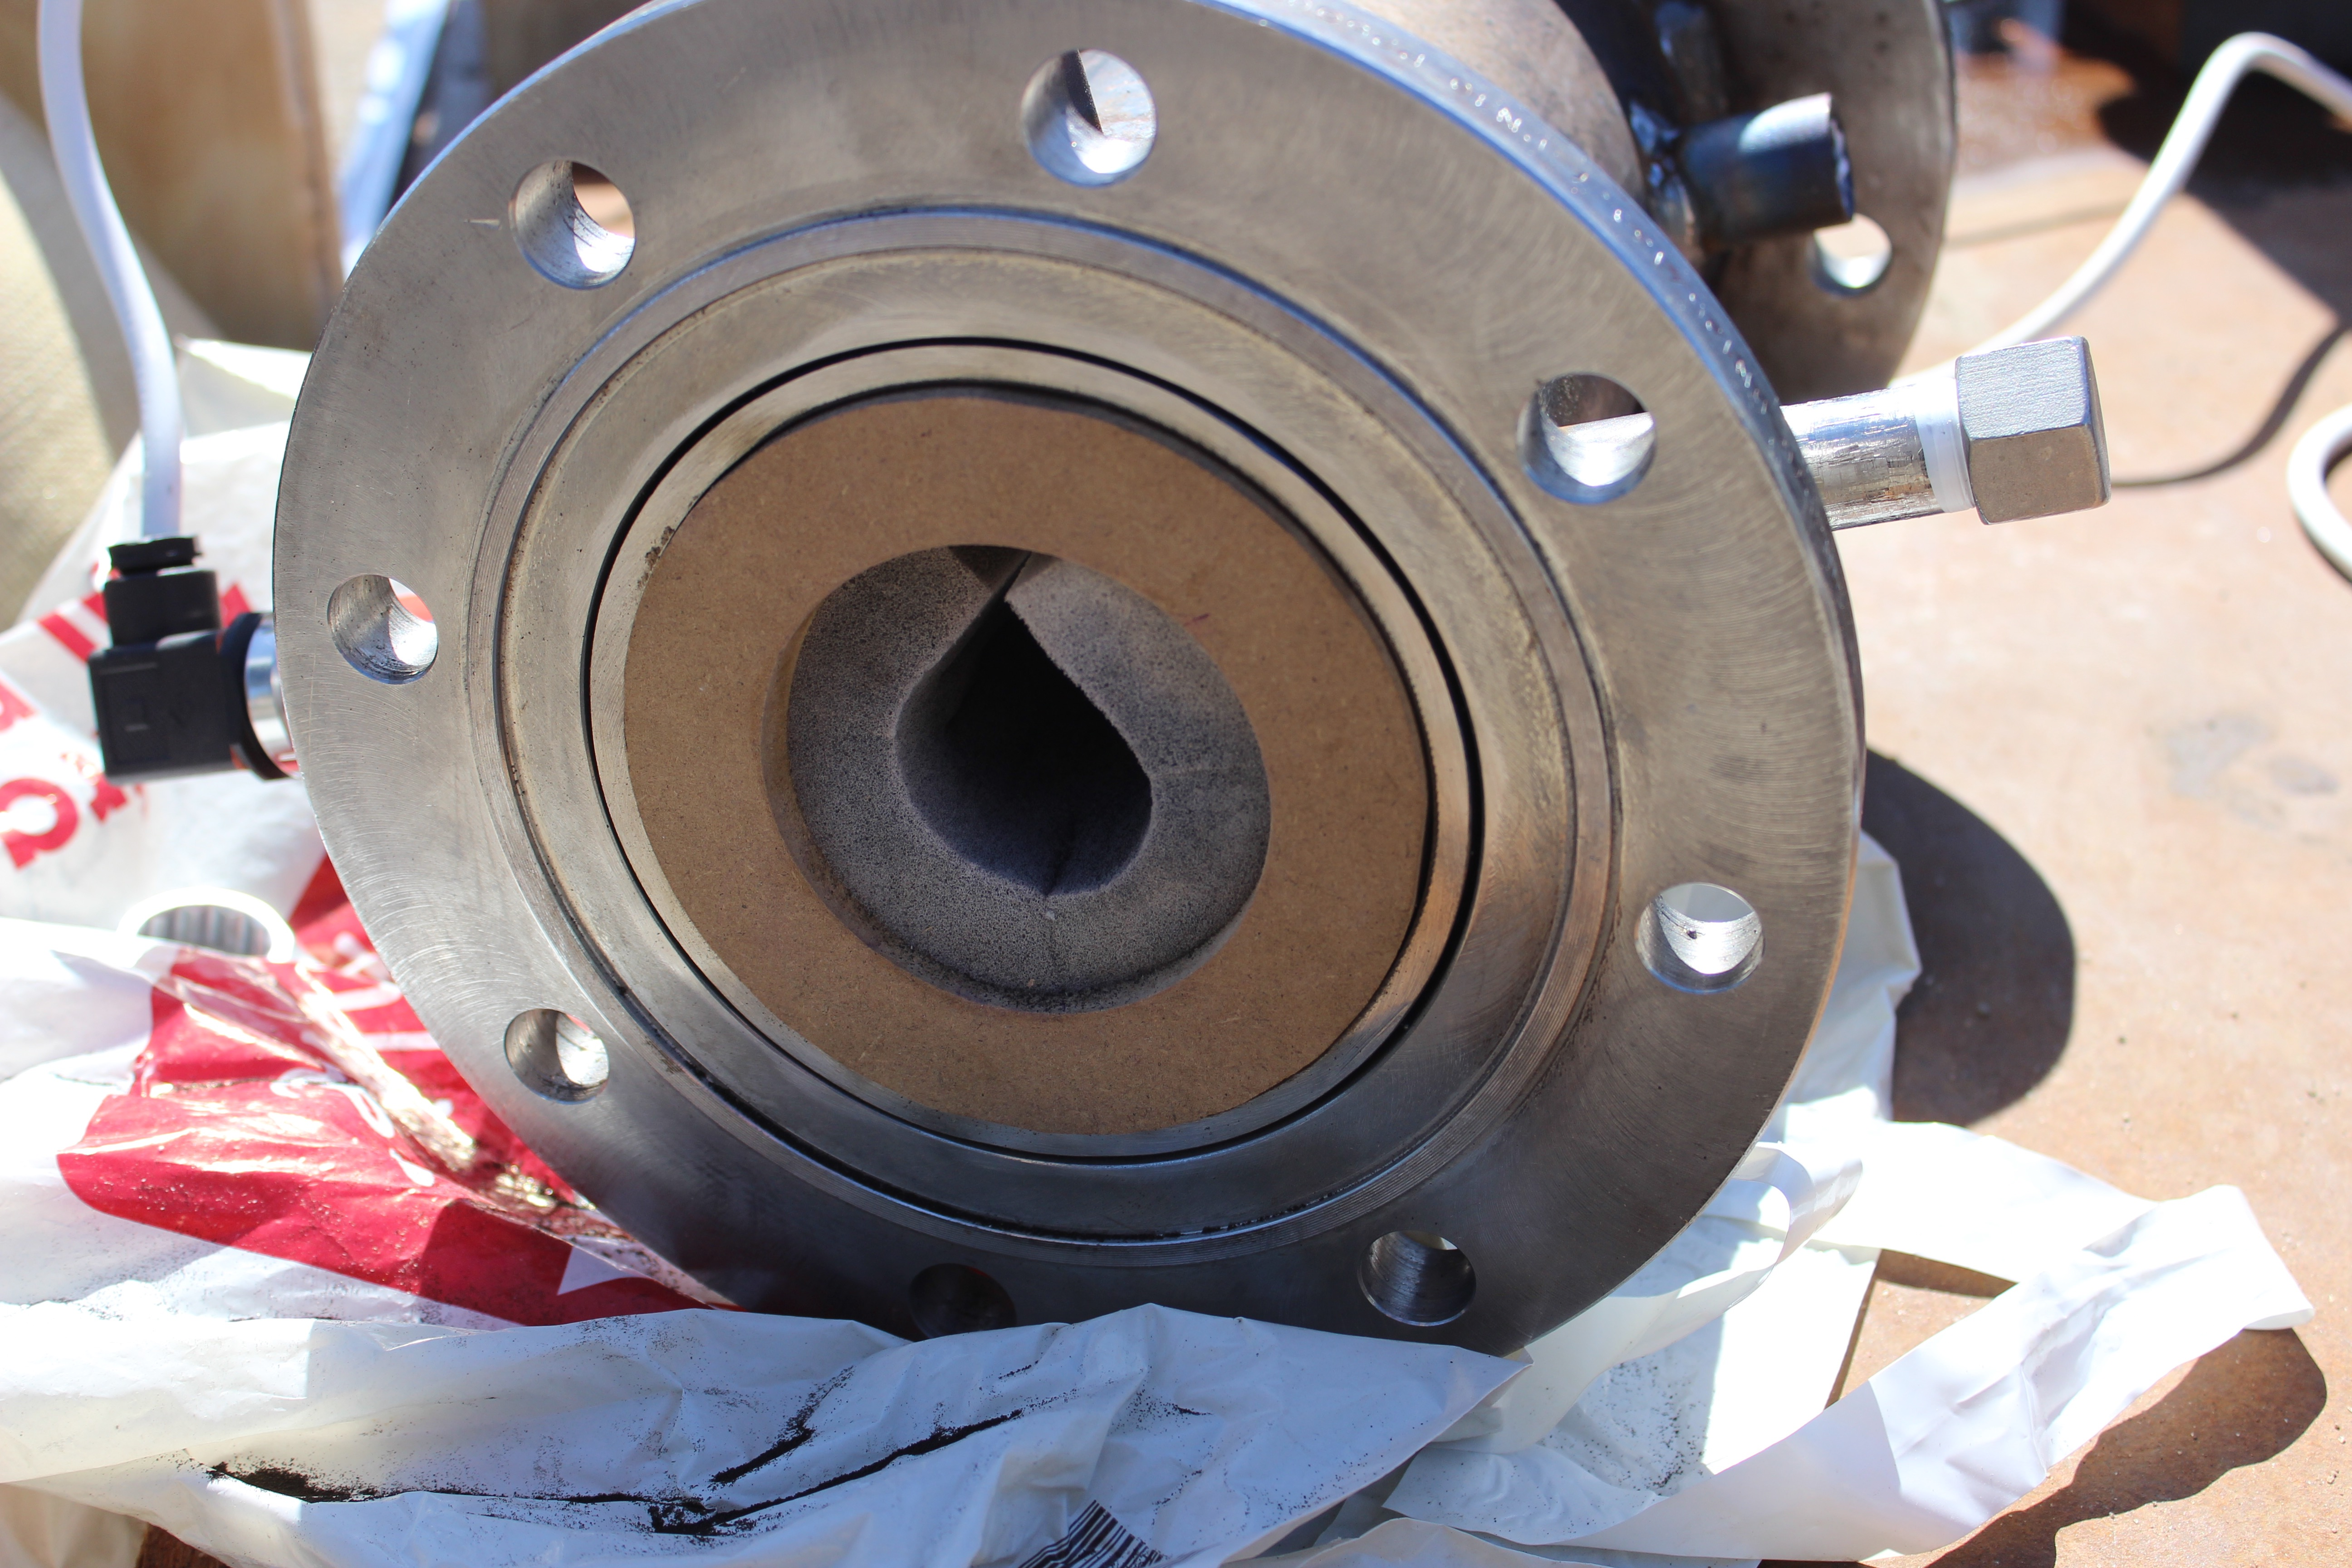
\includegraphics[width=\textwidth]{decompchamber}
			\caption{Foam permeated with \chem{KMnO_4} dust inserted into the decomposition chamber, inside a tube of MDF, in order to avoid accumulation of liquid \chem{H_2 O_2}}
			\label{fig:kmno4foam}
		\end{figure}

		Day 2 started early with preliminary water tests at 12:13, 12:33, 12:57 and 13:21. Two injectors, a low-flow and a high-flow, were brought along and tests of both ensued. Following the preliminary water tests, the rocket chambers were assembled and foam permeated with \chem{KMnO_4} was prepared and inserted into the decomposition chamber, as seen in figure \ref{fig:kmno4foam}. Initial rocket test started almost two hours after the final water test at 15:20 with $\si{1.5}{L}$ of \chem{H_2 O_2} at $\si{24}{bar}$ pressure. After the test, the stand was quite smokey as the rocket flanges were \emph{not} tightened correctly and an O-ring was missing. A leak between the grain's chamber and the after-burn chamber seared the underside of the protective casing, thankfully without harming any of the measurement equipment. After the small upset, three additional tests were carried out. \fxnote{EVT. Lav tabel over tests i stedet for at skrive det}

		The three first tests were all done with the low-flow nozzle with a total radius of $\si{1.5}{mm}$ per injector hole, of which there were three. The final tests were carried out with the large injector with hole radii of $\si{2}{mm}$. The second test happened at 17:22 with a \chem{H_2 O_2} pressure of $\si{24}{bar}$, the next at 18:32 with $\si{31}{bar}$. The final test was done at 20:19, with a \chem{H_2 O_2} pressure of $\si{31}{bar}$, with the high-flow nozzle.

		All tests were done with the same hexagonal patterned grain, with masses pre- and postburn noted.

		The day concluded with Peter Madsen using our test rig to test his own rocket based on a catalytic pack, with no combustion present.

		The firing procedure was meticulously planned out, in order to avoid any eventual dangers. Thus, including a such list is essential for future rocketeers:

\section{Firing Procedure}
Launching the rocket requires several crucial steps in order to safely ignite the engine. Safety is the number one priority, thus, a stepwise checklist is necessary.

PRELAUNCH
\begin{enumerate}
  \itemsep0em
  \item Insert grain
  \item Insert foam permeated with \chem{KMnO_4}
  \item Assemble rocket chambers
  \item Establish remote access to control computer
  \item Ensure measurement options are correct
  \item Check signal and restart ManuWare
  \item Create new data-log file
\end{enumerate}
ALL CLEAR AREA EXCEPT FUEL RESPONSIBLE PERSON
\begin{enumerate}
  \itemsep0em
  \item Equip \chem{H_2 O_2} safety equipment
  \item Fill tank with \chem{H_2 O_2}
  \item Pressurize tank
  \item CLEAR THE AREA
  \item Start data-collection and cameras
  \item Arm the rocket
  \item Fire the rocket
  \item Stop data-collection and cameras
  \item Remove external pressure compressor
  \item Depressurize tank
  \item Area is safe
\end{enumerate}

Peter Madsen and his assistant Stefan Eisenknappl are the only two people present when loading the rocket with \chem{H_2 O_2}. The procedure is executed from start to end at each launch, and has several areas where it can be improved if time permits.

The control computer should be replaced by a microcontroller, such as an arduino or raspberry pi. As of this project, the data bandwidth is too low in either alternative, but it is a viable solution in the near future.

In order to reduce reload time, adding more piping to the christmas tree is necessary, as air leaving the \chem{H_2 O_2} tank flows back, spilling the \chem{H_2 O_2} concentration out of the funnel. When a suitable final design is done, welding the pieces together is a superior alternative to using bolts and nuts. Welding removes any chance hydrogenperoxide leaking, damaging the rocket and measurement equipment.

The rocket's arming and controlpad needs to be set up in a smarter, more convenient way. The ideal setup is to have a single controlbox, that when starts data-collection as soon as the rocket is armed, and notes when it is fired. This would allow everything to be controlled from a single box, with measurements being saved to a raspberry pi situated at the base of the rocket. Data can then instantaneously be read from a secondary computer through cable or wireless connection. As the rocket's final destination is space, continuously improving data-transfer and making the rocket an individual unit is paramount.

Removing additional noise from measurements can easily be done avoiding ground-loops. The ignition controlpad was grounded differently than the other equipment, which introduced another way for electricity to run to ground.

\section{Results}

A total of ten measurements were collected at every test. The most essential is the Piezoelectric pressure sensors located at the front. The simulation calculates the pressure after the combustion chamber, and at the nozzle's exit.

\begin{figure}
	\centering
	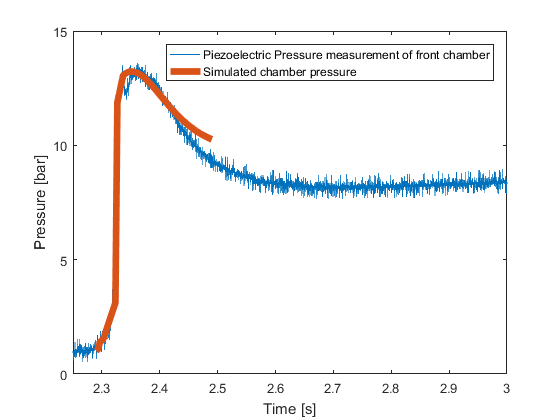
\includegraphics[width=\textwidth]{peakBurn2wsim}
	\caption{The second burn's front chamber peak, as found by the Piezoelectric pressure sensor. Plotted on top is the simulation created in this bachelor's thesis.}
	\label{fig:peakBurn2wsim}
\end{figure}

The experimental and simulation results are seen in figure \ref{fig:peakBurn2wsim}, where the blue line is the experimental results, and the red is the simulated pressure. The simulation assumes no combustion until a temperature of $\si{220}{celcius}$, at which all of the oxygen inside the combustion chamber is instantly consumed, followed by a steady burning phase. The instantaneous combustion looks like an explosion, as more oxygen is available at this point than at any other. The experimental front pressure dips shortly after initial combustion, which may be due to a shockwave moving through the rocket, forcing new oxygen from flowing to the grain's surface for a short period of time. The pressure then drops rapidly to a steady state, at which the simulation ends. Take note of the simlation's timescale, as the duration of the peak is very small, almost only two tenths of a second.


\begin{figure}
	\centering
	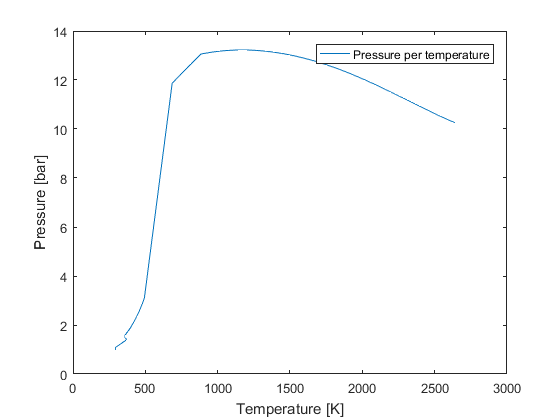
\includegraphics[width=\textwidth]{PperTsimonly}
	\caption{Pressure per temperature plotted over the simulated timespan in figure \ref{fig:peakBurn2wsim}. As the temperature rises, the pressure falls.}
	\label{fig:pressurepertemp}
\end{figure}
